\documentclass[tikz,border=3pt]{standalone}
\usepackage[utf8]{inputenc}
\usepackage[T1]{fontenc}
\usepackage{lmodern}
\renewcommand{\familydefault}{\sfdefault}
\usepackage{sansmath}\sansmath
\usepackage{chemfig}
\usepackage{pgfplots}\pgfplotsset{compat=1.18,/pgf/number format/use comma,/pgf/number format/1000 sep={.}}
\usetikzlibrary{arrows.meta,calc,positioning,decorations.pathmorphing,patterns}
% paleta del sitio
\definecolor{nar}{HTML}{E8680C}\definecolor{narc}{HTML}{FFB35C}\definecolor{hielo}{HTML}{FFF3E8}
\definecolor{tinta}{HTML}{1D1D1F}\definecolor{gris}{HTML}{6E6E73}\definecolor{lila}{HTML}{7C5CF0}
\definecolor{azul}{HTML}{2F6FD6}\definecolor{menta}{HTML}{17A673}\definecolor{coral}{HTML}{E8342A}
\begin{document}
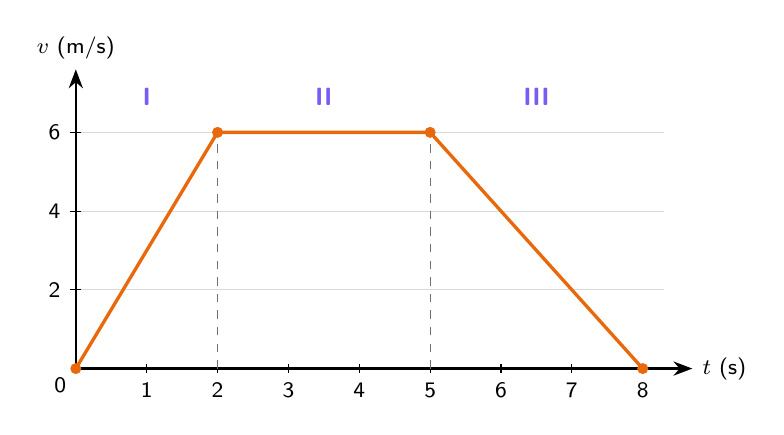
\begin{tikzpicture}[font=\footnotesize,>={Stealth[length=2.4mm]},x=0.9cm,y=0.5cm]
\foreach \y in {2,4,6} \draw[gris!25] (0,\y) -- (8.3,\y);
\draw[->,thick] (0,0) -- (8.7,0) node[right] {$t$ (s)};
\draw[->,thick] (0,0) -- (0,7.6) node[above] {$v$ (m/s)};
\foreach \x in {1,...,8} \draw (\x,0.12) -- (\x,-0.12) node[below] {\x};
\foreach \y in {2,4,6} \draw (0.08,\y) -- (-0.08,\y) node[left] {\y};
\node[below left] at (0,0) {0};
\draw[dashed,gris] (2,0) -- (2,6) (5,0) -- (5,6);
\draw[very thick,nar] (0,0) -- (2,6) -- (5,6) -- (8,0);
\fill[nar] (0,0) circle (2pt) (2,6) circle (2pt) (5,6) circle (2pt) (8,0) circle (2pt);
\node[font=\small\bfseries,lila] at (1,6.9) {I};
\node[font=\small\bfseries,lila] at (3.5,6.9) {II};
\node[font=\small\bfseries,lila] at (6.5,6.9) {III};
\end{tikzpicture}
\end{document}
